\documentclass[12pt,a4paper]{article}
\usepackage[T1]{fontenc}
\usepackage[left=2cm, right=2cm, top=2cm, bottom=2cm]{geometry}
\usepackage{graphicx}
\usepackage{mathtools}
\usepackage{amssymb}
\usepackage{amsthm}
\usepackage{hyperref}
\usepackage{braket}
\usepackage{setspace}
\usepackage{paralist}
\usepackage{nicefrac}
\usepackage{siunitx}
\usepackage{tikz}

\title{On few-state (VB-$n$CT) theory}
\author{Pierre Beaujean}

\allowdisplaybreaks
\onehalfspacing

\begin{document}
	\maketitle
	
	\section{Introduction}
	
In nonlinear optics (NLO), promising molecular architectures often belong to the push-pull family. These structures typically consist of electron donor and acceptor groups connected by a $\pi$-conjugated segment that facilitates electronic ``communication'' between the two moieties.

To elucidate the relationships between NLO properties and structure, simplified models have been developed to capture complex phenomena with minimal parameters. The valence-bond charge-transfer (VB-CT) model, pioneered by Mulliken \cite{mullikenMolecularCompoundsTheir1952}, has been particularly successful in describing the first hyperpolarizabilities of push-pull polyenes. It also applies to other properties, such as UV/VIS absorption spectra and various physico-chemical characteristics \cite{benderTheoreticalModelsChargetransfer1986}. This model represents a system as a superposition of two limiting states, a valence-bond state, $\phi_{VB}$, and a charge-transfer state, $\phi_{CT}$, connected by electron displacement from the donor to the acceptor (see Fig.~\ref{sc:vbct}). Using fundamental parameters, such as the ionization energy of the donor, electron affinity of the acceptor, and the coupling between these states, the VB-CT model provides valuable insight into structure-activity relationships.  Indeed, when combined with the sum-over-states (SOS) theory developed by Orr and Ward \cite{orrPerturbationTheoryNonlinear1971}, these models provide estimate of NLO properties and identification of valuable structure-activity relationships.


\begin{figure}[!h]
	\centering
	\includegraphics[width=.5\linewidth]{Scheme1}
	\caption{Limiting forms of the VB-CT model.}
	\label{sc:vbct}
\end{figure}

Despite its simplicity, this model has proven versatile, allowing extensions to systems with multiple donor/acceptor groups through 3-state \cite{hahnNonlinearOpticalProperties1999,barzoukasMolecularEngineeringPush2000,yangLargeOffDiagonalContribution2003}, 4-state \cite{choElementaryDescriptionNonlinear1998}, and 5-state \cite{choNonlinearOpticalProperties2002} descriptions.
The goal of this document is to quickly review theses models few-state models and to introduce a few useful relationships.

\section{Theory}

\subsection{A model Hamiltonian}\label{sec:hamiltonian}

Given a set of basis functions $\{\phi_i\}$, the energy of a trial function $\Psi = \sum_i c_i \phi_i$ is always greater than or equal to the true ground state energy, $\varepsilon_0$:\begin{equation*}
	 \varepsilon_0 \leq \varepsilon, \text{ where } \varepsilon = \frac{\braket{\Psi|H|\Psi}}{\braket{\Psi|\Psi}},
\end{equation*}
One minimizes the energy of the trial function by setting $\frac{d\varepsilon}{dc_i} = 0$. 
This yields a set of so-called secular equations of the form:\begin{equation}
	\forall k: \sum_i c_i (H_{ki} - \varepsilon_k S_{ki}) = 0, 
\end{equation}
where $S_{ki} = \braket{\phi_k | \phi_i}$ (overlap matrix) and $H_{ki} = \braket{\phi_k | \hat{H} | \phi_i}$ (Hamiltonian matrix). 
This is a generalized eigenvalue problem. 
If the basis functions are orthogonal, i.e., $S_{ki} = \delta_{k,i}$, this reduces to a standard eigenvalue problem, $HC=C\varepsilon$, where diagonalizing $H$ gives the energy levels, $\varepsilon$. $C$ is the matrix of coefficients, also referred to as the eigenfunctions of the system.

In the VB-$n$CT framework, corresponding to a $(n+1)$-state model, a set of orthogonal functions is employed consisting of one valence-bond (VB) state, $\phi_{VB}$, and $n$ charge-transfer (CT) states, $\{\phi_{CT,i}|0<i\leq n\}$. This leads to a model Hamiltonian, given by a $(n+1)\times(n+1)$ matrix and parameterized as follows:
\begin{align}
	&\braket{\phi_{VB}|\hat{H}|\phi_{VB}} = E_{VB}, 
	\braket{\phi_{VB}|\hat{H}|\phi_{CT,i}} = t, \text{ and } 
	\braket{\phi_{CT,i}|\hat{H}|\phi_{CT,j}} = \begin{cases}
		E_{CT} & \text{if } i=j,\\
		T & \text{otherwise},
	\end{cases}\label{eq:hamilonian}
\end{align}
where $E_{VB}$ and $E_{CT}$ denote the energies of the VB and CT states, respectively, while $t$ and $T$ are the transfer integrals. 

Solving the eigenvalue problem yields a ground state, $\ket{0}$, with minimal energy, a set of $(n-1)$-fold degenerate excited states, $\{\ket{e_i} | 0<i< n\}$ (which does not exists when $n=1$), and a single non-degenerate excited state, $\ket{f}$.
Corresponding eigenvalues were provided by Cho \emph{et al.} \cite{choNonlinearOpticalProperties2002} and are, in all generality, given by:
\begin{align}
	E_{0} &= \frac{1}{2} \left[E_{VB} + E_{CT} - (n-1)T - \sqrt{(V - (n-1)T)^2 + 4nt^2}\right], \nonumber\\
	E_{e_i} &= E_{CT} + T, \nonumber\\
	E_{f} &= \frac{1}{2} \left[E_{VB} + E_{CT} - (n-1)T + \sqrt{(V - (n-1)T)^2 + 4nt^2}\right],
\end{align}
where $V = E_{CT} - E_{VB}$. 
The associated eigenfunctions are:
\begin{align}
	\ket{0} &= \cos\delta\,\ket{\phi_{VB}} + \frac{\sin\delta}{\sqrt{n}} \sum_{0<j\leq n} \ket{\phi_{CT,j}},\nonumber\\
	\ket{e_i} &= \frac{1}{\sqrt{i(i+1)}}\left[i \ket{\phi_{CT,i+1}} - \sum_{0<j\leq i} \ket{\phi_{CT,j}}\right],\nonumber\\
	\ket{f} &= \sin\delta\,\ket{\phi_{VB}} - \frac{\cos\delta}{\sqrt{n}} \sum_{0<j\leq n} \ket{\phi_{CT,j}},
\end{align}
where the mixing angle $\delta \in [0, \nicefrac{\pi}{2}]$ is introduced. For $0 \leq \delta < \nicefrac{\pi}{4}$, the ground state is VB-dominated, whereas for $\nicefrac{\pi}{4} < \delta \leq \nicefrac{\pi}{2}$, the CT state dominates. The point $\delta = \nicefrac{\pi}{4}$ is referred to as the \textit{cyanine limit}.

Minimizing the ground-state energy $E_g$ with respect to $\delta$ provides a condition linking the parameters:
\begin{equation}
	\frac{\partial E_g(\delta)}{\partial \delta} = 0 \Rightarrow V - (n-1)T = 2t \sqrt{n} \cot(2\delta). \label{eq:cot}
\end{equation}
Setting the energy origin to:
\begin{equation}
	E_{VB} + E_{CT} - (n-1)T = 0, \label{eq:eorig}
\end{equation}
simplifies the eigenvalues to:
\begin{align}
	E_{0} = -\sqrt{n} \frac{t}{\sin(2\delta)}, E_{e_i} = nT + t \sqrt{n} \cot(2\delta), \text{ and }
	E_{f} =  \frac{t}{\sin(2\delta)}\sqrt{n}.\label{eq:energies}
\end{align}

To monitor variations in molecular properties, the charge-transfer (CT) character of the ground state, $\ell_{CT}$, can be introduced as follows \cite{choNonlinearOpticalProperties2002,choElementaryDescriptionNonlinear1998,yangLargeOffDiagonalContribution2003}:
\begin{equation}
	\ell_{CT} = \frac{1}{n} \sin^2 \delta.
\end{equation}
With $\delta \in [0, \nicefrac{\pi}{2}]$, $\ell_{CT}$ varies in the range $\ell_{CT} \in [0, \nicefrac{1}{n}]$. A value of $\ell_{CT} = 0$ indicates a ground state fully described by the VB form, while $\ell_{CT} = \nicefrac{1}{n}$ corresponds to a state entirely characterized by CT. 
An additional parameter, introduced by Barzoukas and collaborators \cite{barzoukasTWOFORMDESCRIPTIONPUSHPULL1996,barzoukasTwostateDescriptionHyper1996,blanchard-desceTwoformTwostateAnalysis1998a}, measures the VB-CT mixing:
\begin{equation}
	m_{CT} = -\cos(2\delta) = 2n \ell_{CT} - 1.
\end{equation} 
This parameter, $m_{CT}$, ranges from $-1$ (VB-dominated) to $+1$ (CT-dominated), effectively capturing the balance between VB and CT character in the ground state.

\subsection{A set of dipole moments}\label{sec:dipoles}

To utilize the SOS expression, both excitation energies (calculated, in the VB-$n$CT model, as differences between eigenvalues, given in Eq.~\eqref{eq:energies}) and transition dipoles are required. In general, transition dipoles are computed as follows:
\begin{equation}
	\vec{\mu}_{ij} = \braket{i | \hat{\mu} | j} = \sum_{\nu \kappa} (C_{i \nu})^\dagger C_{j \kappa} \, \braket{\phi_\nu | \hat{\mu} | \phi_\kappa},
\end{equation}
where $\ket{i} = \sum_\nu C_{i \nu} \, \ket{\phi_\nu}$ represents the electronic states of the system, $C_{i \nu}$ are the coefficients in the state expansion, and $\ket{\phi_\nu}$ are the basis functions. 

In the VB-$n$CT model, the dipole matrix elements $M_{\mu \nu} = \braket{\phi_\nu | \hat{\mu} | \phi_\kappa}$ are given as follows \cite{luValenceBondChargeTransferModel1994}:
\begin{align}
	\braket{\phi_{VB} | \hat{\mu} | \phi_{VB}} = \braket{\phi_{VB} | \hat{\mu} | \phi_{CT,i}} = 0,
	\braket{\phi_{CT,i} | \hat{\mu} | \phi_{CT,j}} = 
	\begin{cases}
		\vec{\mu}_{CT,i} & \text{if } i = j, \\
		0 & \text{otherwise}.
	\end{cases}
\end{align}
This results in a sparse, diagonal dipole matrix parameterized by a select set of CT dipole moments associated to each CT state, $\{\vec{\mu}_{CT,i} \mid 0 < i \leq n\}$.


\subsection{Parameterization of a VB-$n$CT model} \label{sec:param}

As outlined in Sections \ref{sec:hamiltonian} and \ref{sec:dipoles}, a VB-$n$CT model is uniquely defined by a set of $n$ CT dipole moments, $\{\vec{\mu}_{CT,i} \mid 0 < i \leq n\}$, and either of the following parameterizations:
\begin{enumerate}
	\item Using Eq.~\eqref{eq:hamilonian}: specified by $E_{VB}$, $E_{CT}$ (or equivalently $V$), $t$, and $T$;
	\item Alternatively, by applying the conditions in Eqs.~\eqref{eq:cot} and \eqref{eq:eorig}: specified by $t$, $T$, and one of the mixing parameters defined in Section \ref{sec:hamiltonian} (such as $\delta$, $\ell_{CT}$, or $m_{CT}$).
\end{enumerate}
This allows a straightforward implementation of this model in Python, which outputs excitation energies and transition dipole moments.


\clearpage
\appendix
\setcounter{equation}{0} 
\renewcommand{\theequation}{A\arabic{equation}}

\section{Practical expressions for static $\beta$}

Let's assume the parameterization from Section \ref{sec:param} (with $m_{CT}$ as the mixing parameter), and a (non-divergent) SOS expression  for the static $\beta$ tensor elements \cite{bishopExplicitNondivergentFormulas1994}:\begin{equation}
	\beta_{(\zeta\eta\kappa)} = \hbar^{-2} \sum_\mathcal{P} \sum_{a_1', a_2'} \frac{(\zeta\bar{\eta}\kappa)_{a_1 a_2}}{\omega_{a_1}\,\omega_{a_2}},\label{eq:sos}
\end{equation}
where $\zeta, \eta, \kappa$ are the Cartesian coordinates $x, y, z$ (in the molecular frame, the parenthesis indicates that one can freely permute the indices), $(\zeta\bar{\eta}\kappa)_{a_1 a_2}$ is the notation of Bishop for the product of transition dipole moments, $\sum_{a_1', a_2'}$ is a sum over the $n$ excited states, and $\sum_{\mathcal{P}}$ is the sum over the different permutations. On that ground, one  can derive practical expressions for the components of $\beta$ in different cases, presented below. For an in-depth derivation, see Chapter 11 of Ref.~\cite{mythesis} and the references therein.

\paragraph{2-state ($C_{\infty v}$) model.} These systems consist of a donor-acceptor (D/A) pair typically located at the ends of a $\pi$-conjugated linker, oriented along the $z$-axis for convenience. Assuming that the CT dipole moment, $\mu_{CT}$, lies entirely along the $z$-axis, one obtains the following expression for the only non-null component, $\beta_{zzz}$ \cite{barzoukasTWOFORMDESCRIPTIONPUSHPULL1996,barzoukasTwostateDescriptionHyper1996,blanchard-desceTwoformTwostateAnalysis1998a}:
\begin{align}
	\beta_{zzz} = -\frac{3}{8}\,m_{CT}\,(1 - m_{CT}^2)^2\,\frac{\mu_{CT}^3}{t^2}. \label{eq:2state}
\end{align}


\paragraph{3-state ($C_{2v}$) model.} Assuming that the two CT axes form an angle $\theta\in[0,\nicefrac{\pi}{2}]$ from the $z$ axis \cite{yangLargeOffDiagonalContribution2003}, as represented in Fig.~\ref{sc:mu}, one has:\begin{equation}
	\vec\mu_{CT,1} = \mu_{CT}\,(\sin\theta,0,\cos\theta) \text{ and } \vec\mu_{CT,2} = \mu_{CT}\,(-\sin\theta,0,\cos\theta). 
\end{equation}
There are only two non-null independent components: $\beta_{zzz}$ and  $\beta_{(zxx)}$:\begin{align}
	\beta_{zzz} &= -\frac{3}{16}\,m_{CT}\,(1-m_{CT}^2)^2\,\frac{\mu_{CT}^3}{t^2}\,\cos^3\theta,\nonumber\\
	\beta_{(zxx)} &= \frac{1-m_{CT}^2}{2}\,\mu_{CT}^3\,\sin^2\theta\cos\theta\nonumber\\
	&\hspace{1cm}\times\left\{\frac{1}{\left(2T + t\,\left[2\,\frac{1-m_{CT}}{1+m_{CT}}\right]^{\nicefrac{1}{2}}\right)^2} + \frac{2}{2t\,\left[\frac{2}{1-m_{CT}^2}\right]^{\nicefrac{1}{2}}\,\left(2T + t\,\left[2\,\frac{1-m_{CT}}{1+m_{CT}}\right]^{\nicefrac{1}{2}}\right)}\right\}.\label{eq:3state}
\end{align}
Note that when $\theta=\SI{90}{°}$, both $\beta_{zzz}$ and $\beta_{(zxx)}$ goes to zero, since it corresponds to a situation with a center of inversion ($D_{\infty h}$). 


\begin{figure}[!h]
	\centering
	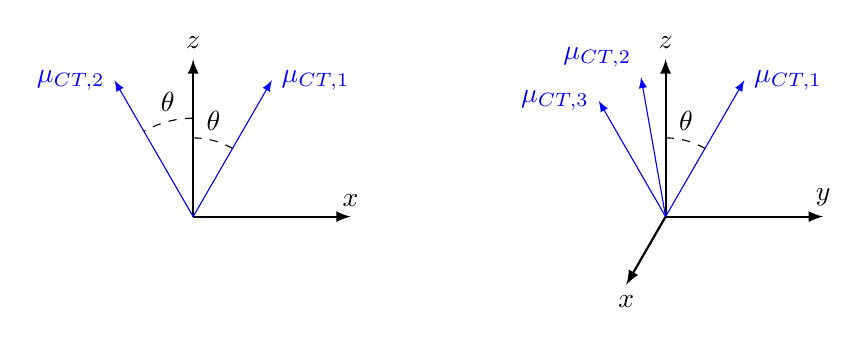
\begin{tikzpicture}
		\begin{scope}
			\draw[-latex,thick] (0,0) -- +(0,2) node[above]{$z$};
			\draw[-latex,thick] (0,0) -- +(2,0) node[above]{$x$};
			\draw[-latex,blue] (0,0) -- (60:2) node[right]{$\mu_{CT,1}$};
			\draw[dashed] (0,1) arc(90:60:1) node[midway,above]{$\theta$};
			\draw[-latex,blue] (0,0) -- (120:2) node[left]{$\mu_{CT,2}$};
			\draw[dashed] (0,1.25) arc(90:120:1.25) node[midway,above]{$\theta$};
		\end{scope}
		 \begin{scope}[xshift=6cm]
		 	\draw[-latex,thick] (0,0) -- +(0,2) node[above]{$z$};
		 	\draw[-latex,thick] (0,0) -- +(2,0) node[above]{$y$};
		 	\draw[-latex,thick] (0,0) -- +(-120:1) node[below]{$x$};
		 	\draw[-latex,blue] (0,0) -- (60:2) node[right]{$\mu_{CT,1}$};
		 	\draw[dashed] (0,1) arc(90:60:1) node[midway, above]{$\theta$};
		 	\draw[-latex,blue] (0,0) -- (100:1.8) node[anchor=south east]{$\mu_{CT,2}$};
		 	\draw[-latex,blue] (0,0) -- (120:1.7) node[left]{$\mu_{CT,3}$};
		 \end{scope}
	\end{tikzpicture}
	\caption{Representation of the charge-transfer dipoles ($\mu_{CT}$) in the 3-state (left) and 4-state (right) models.}
	\label{sc:mu}
\end{figure}

\paragraph{4-state ($C_{3v}$) system.} Let's, this time, assume that the three dipole moments are at \SI{120}{\degree} from each other in the $xy$ plane (and the first one point to the $y$ direction), but that there is a $\theta\in[0,\nicefrac{\pi}{2}]$ angle between the dipoles and the $z$ axis, as in Fig.~\ref{sc:mu}. Thus,\begin{equation}
	\vec\mu_{CT,1} = \mu_{CT}\,(0,\sin\theta,\cos\theta), \vec\mu_{CT,2} = \vec\mu_{CT,3} = \frac{\mu_{CT}}{2}\,(\pm\sqrt{3}\,\sin\theta, -\sin\theta, 2\,\cos\theta)
\end{equation}
There are three non-null independent components: $\beta_{zzz}$,  $\beta_{(zyy)}$, and $\beta_{yyy}$. Their expressions are:\begin{align}
	\beta_{zzz} &= -\frac{1}{8}\,m_{CT}\,(1-m_{CT}^2)^2\,\frac{\mu^3_{CT}}{t^2}\,\cos^3\theta,\nonumber\\
	\beta_{(zyy)} &= \frac{1-m_{CT}^2}{4}\,\mu_{CT}^3\,\sin^2\theta\cos\theta\nonumber\\
	&\hspace{1cm}\times\left\{\frac{1}{\left(3T + t\,\left[3\,\frac{1-m_{CT}}{1+m_{CT}}\right]^{\nicefrac{1}{2}}\right)^2} + \frac{2}{2t\,\left[\frac{3}{1-m_{CT}^2}\right]^{\nicefrac{1}{2}}\,\left(3T + t\,\left[3\,\frac{1-m_{CT}}{1+m_{CT}}\right]^{\nicefrac{1}{2}}\right)}\right\},\nonumber\\
	\beta_{yyy} &= \frac{3}{4}\,(1+m_{CT})\,\frac{\mu_{CT}^3}{\left(3T + t\,\left[3\,\frac{1-m_{CT}}{1+m_{CT}}\right]^{\nicefrac{1}{2}}\right)^2}\,\sin^3\theta.\label{eq:4state}
\end{align}
The relationship $\beta_{yyy} = -\beta_{(yxx)}$ holds in this model,\footnote{Symmetry tables generally reports  $\beta_{yyy} = -\beta_{(yyx)}$, but it is just a matter of defining the $\sigma_v$. Also, this definition is consistent with $D_{3h}$.} as expected from $C_{3v}$ symmetry. Note that when $\theta=\SI{90}{°}$, the system correspond to a $D_{3h}$ symmetry, with $\beta_{zzz} = \beta_{(zyy)} = \beta_{(zxx)} = 0$.

\paragraph{5-states ($T_d$) system.} For the sake of completeness, lets finally consider the $T_d$ geometry, which was first reviewed by Cho \emph{et al.} \cite{choNonlinearOpticalProperties2002}. The dipole moments are (arbitrarily) given by\begin{align}
	&\vec\mu_{CT,1} = \mu_{CT}\,\frac{\sqrt{3}}{3}\,(1, 1, 1), \vec\mu_{CT,2} = \mu_{CT}\,\frac{\sqrt{3}}{3}\,(1, -1, -1), \nonumber\\
	&\hspace{1cm}\vec\mu_{CT,3} = \mu_{CT}\,\frac{\sqrt{3}}{3}\,(-1, -1, 1), \text{ and } \vec\mu_{CT,4} = \mu_{CT}\,\frac{\sqrt{3}}{3}\,(-1, 1, -1).
\end{align}
In this case, there is only one non-null independent component:\begin{equation}
	\beta_{(xyz)} = (1+m_{CT})\,\frac{\sqrt{3}}{3}\frac{\mu_{CT}^3}{\left(4T + 2t\,\left[\frac{1-m_{CT}}{1+m_{CT}}\right]^{\nicefrac{1}{2}}\right)^2}.\label{eq:5state}
\end{equation}


\bibliographystyle{unsrt}
\bibliography{biblio}
	
\end{document}